\chapter{Conception Détaillée du Système}

\section{Introduction}

Ce chapitre présente la conception détaillée du système SmartClub Analytics à travers des diagrammes UML complets. Nous détaillons l'architecture des modules, les modèles de données, les flux de communication, et les interactions entre les différents composants du système.

\section{Diagramme de Classes UML}

\subsection{Modèle de Données Principal}

Le diagramme de classes ci-dessous illustre la structure des données persistantes du système :

\begin{figure}[H]
\centering
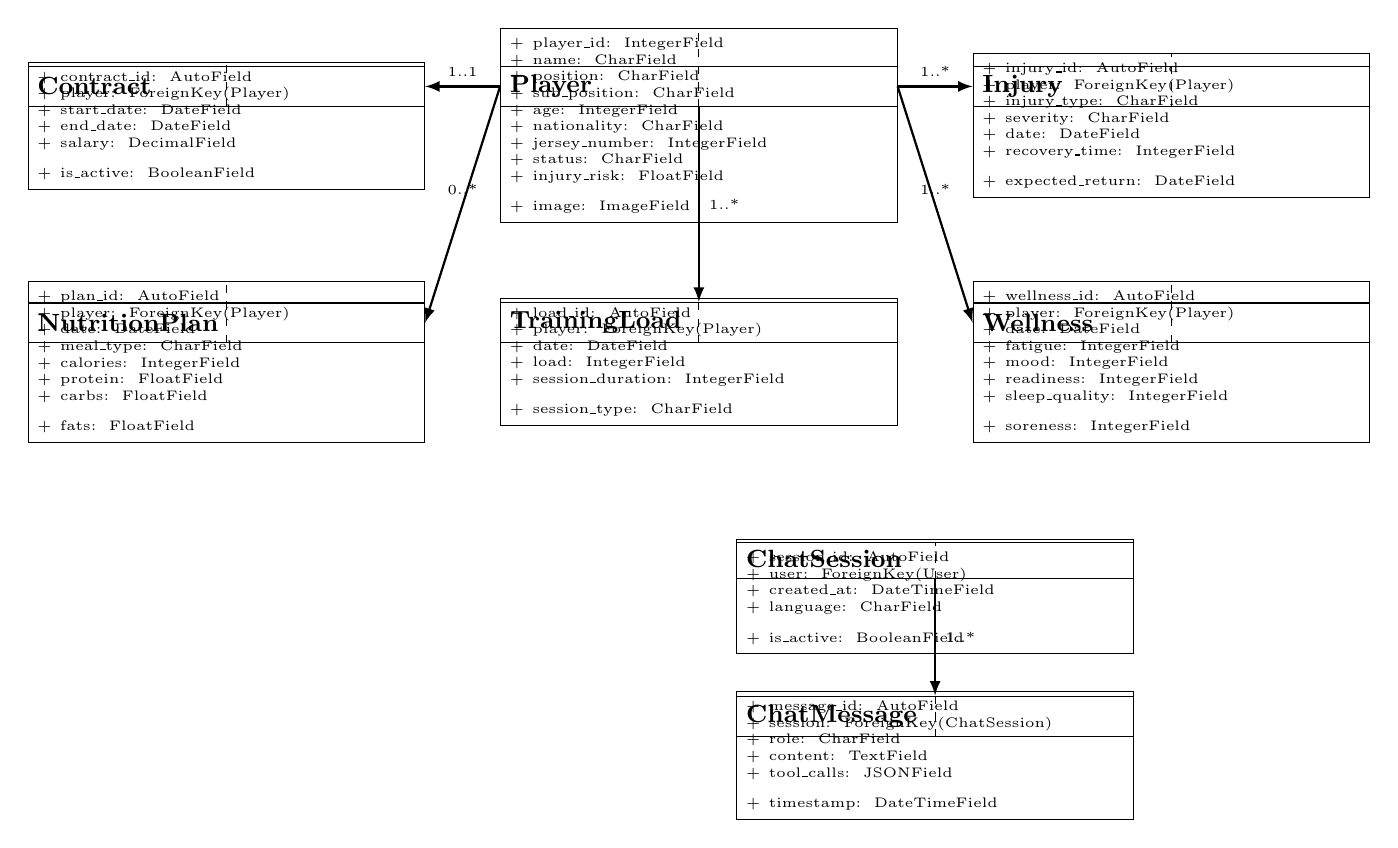
\begin{tikzpicture}[
    cls/.style={rectangle, draw, minimum width=5cm, minimum height=0.5cm, text width=4.8cm, font=\small},
    relationship/.style={-latex, thick}
]

% Classe Player
\node[cls] (player) at (0,0) {\textbf{Player}};
\node[cls] (playerattr) at (0,-0.5) {\tiny + player\_id: IntegerField \\ + name: CharField \\ + position: CharField \\ + sub\_position: CharField \\ + age: IntegerField \\ + nationality: CharField \\ + jersey\_number: IntegerField \\ + status: CharField \\ + injury\_risk: FloatField \\ + image: ImageField};
\draw[dashed] (player.south) -- (playerattr.north);

% Classe Injury
\node[cls] (injury) at (6,0) {\textbf{Injury}};
\node[cls] (injuryattr) at (6,-0.5) {\tiny + injury\_id: AutoField \\ + player: ForeignKey(Player) \\ + injury\_type: CharField \\ + severity: CharField \\ + date: DateField \\ + recovery\_time: IntegerField \\ + expected\_return: DateField};
\draw[dashed] (injury.south) -- (injuryattr.north);

% Classe Contract
\node[cls] (contract) at (-6,0) {\textbf{Contract}};
\node[cls] (contractattr) at (-6,-0.5) {\tiny + contract\_id: AutoField \\ + player: ForeignKey(Player) \\ + start\_date: DateField \\ + end\_date: DateField \\ + salary: DecimalField \\ + is\_active: BooleanField};
\draw[dashed] (contract.south) -- (contractattr.north);

% Classe TrainingLoad
\node[cls] (training) at (0,-3) {\textbf{TrainingLoad}};
\node[cls] (trainingattr) at (0,-3.5) {\tiny + load\_id: AutoField \\ + player: ForeignKey(Player) \\ + date: DateField \\ + load: IntegerField \\ + session\_duration: IntegerField \\ + session\_type: CharField};
\draw[dashed] (training.south) -- (trainingattr.north);

% Classe Wellness
\node[cls] (wellness) at (6,-3) {\textbf{Wellness}};
\node[cls] (wellnessattr) at (6,-3.5) {\tiny + wellness\_id: AutoField \\ + player: ForeignKey(Player) \\ + date: DateField \\ + fatigue: IntegerField \\ + mood: IntegerField \\ + readiness: IntegerField \\ + sleep\_quality: IntegerField \\ + soreness: IntegerField};
\draw[dashed] (wellness.south) -- (wellnessattr.north);

% Classe NutritionPlan
\node[cls] (nutrition) at (-6,-3) {\textbf{NutritionPlan}};
\node[cls] (nutritionattr) at (-6,-3.5) {\tiny + plan\_id: AutoField \\ + player: ForeignKey(Player) \\ + date: DateField \\ + meal\_type: CharField \\ + calories: IntegerField \\ + protein: FloatField \\ + carbs: FloatField \\ + fats: FloatField};
\draw[dashed] (nutrition.south) -- (nutritionattr.north);

% Classe ChatSession
\node[cls] (chat) at (3,-6) {\textbf{ChatSession}};
\node[cls] (chatattr) at (3,-6.5) {\tiny + session\_id: AutoField \\ + user: ForeignKey(User) \\ + created\_at: DateTimeField \\ + language: CharField \\ + is\_active: BooleanField};
\draw[dashed] (chat.south) -- (chatattr.north);

% Classe ChatMessage
\node[cls] (msg) at (3,-8) {\textbf{ChatMessage}};
\node[cls] (msgattr) at (3,-8.5) {\tiny + message\_id: AutoField \\ + session: ForeignKey(ChatSession) \\ + role: CharField \\ + content: TextField \\ + tool\_calls: JSONField \\ + timestamp: DateTimeField};
\draw[dashed] (msg.south) -- (msgattr.north);

% Relations
\draw[relationship] (player.east) -- node[above]{\tiny 1..*} (injury.west);
\draw[relationship] (player.west) -- node[above]{\tiny 1..1} (contract.east);
\draw[relationship] (player.south) -- node[right]{\tiny 1..*} (training.north);
\draw[relationship] (player.east) -- node[above]{\tiny 1..*} (wellness.west);
\draw[relationship] (player.west) -- node[above]{\tiny 0..*} (nutrition.east);
\draw[relationship] (chat.south) -- node[right]{\tiny 1..*} (msg.north);

\end{tikzpicture}
\caption{Diagramme de classes UML du modèle de données}
\label{fig:class-diagram}
\end{figure}

\subsection{Modèle de Données pour le Module IA}

Le module IA utilise une structure de données spécifique pour l'apprentissage automatique :

\begin{itemize}
    \item \textbf{AbsenceDaysDataset} : Historique des absences des joueurs avec caractéristiques (position, âge, charge d'entraînement, historique de blessures).
    \item \textbf{InjuryRiskDataset} : Caractéristiques d'entraînement et de bien-être étiquetées avec le risque de blessure réel.
    \item \textbf{Features ML} : ACWR (28j/7j), monotonicité de charge, strain, fatigue cumulée, qualité du sommeil.
\end{itemize}

\section{Diagrammes de Séquence}

\subsection{Authentification et Connexion}

\begin{figure}[H]
\centering
\begin{tikzpicture}[
    actor/.style={rectangle, draw, minimum width=2cm, minimum height=0.8cm, font=\small},
    line/.style={-latex, thick},
    time/.style={dashed}
]

% Lignes de vie
\node[actor] (user) at (-4,0) {Utilisateur};
\node[actor] (front) at (-1,0) {Frontend};
\node[actor] (back) at (2,0) {Backend};
\node[actor] (db) at (5,0) {BDD};

% Séquence
\draw[time] (-4,-1) -- (5,-1);
\draw[time] (-4,-2.5) -- (5,-2.5);
\draw[time] (-4,-4) -- (5,-4);
\draw[time] (-4,-5.5) -- (5,-5.5);
\draw[time] (-4,-7) -- (5,-7);
\draw[time] (-4,-8) -- (5,-8);

% Étapes
\draw[line] (user) -- node[above,font=\tiny] {1. Credentials} (front);
\draw[line] (front) -- node[above,font=\tiny] {2. POST /api/token/} (back);
\draw[line] (back) -- node[above,font=\tiny] {3. Vérification} (db);
\draw[line] (db) -- node[above,font=\tiny] {4. Validé} (back);
\draw[line] (back) -- node[above,font=\tiny] {5. JWT Token} (front);
\draw[line] (front) -- node[above,font=\tiny] {6. Stockage} (user);

\end{tikzpicture}
\caption{Diagramme de séquence du flux d'authentification JWT}
\label{fig:auth-seq}
\end{figure}

\subsection{Assistant IA Conversationnel}

Le flux d'interaction avec l'assistant IA est le plus complexe du système :

\begin{enumerate}
    \item L'utilisateur envoie un message en langage naturel via l'interface React.
    \item Le frontend envoie une requête POST à l'endpoint \texttt{/api/chat-llm/stream/} avec le message et l'historique.
    \item Le backend initialise l'agent LLM avec le contexte approprié (langue, historique).
    \item L'agent envoie la requête au modèle Llama 3.1 via l'API Groq.
    \item Le LLM analyse la requête et décide d'appeler un outil spécifique (ex: \texttt{squad\_risk}, \texttt{player\_search}).
    \item Le backend exécute l'outil (requête à la base de données ou calcul ML).
    \item Le résultat de l'outil est renvoyé au LLM pour synthèse.
    \item Le LLM formule une réponse en langage naturel.
    \item La réponse est streamée vers le frontend via Server-Sent Events (SSE).
\end{enumerate}

\begin{figure}[H]
\centering
\begin{tikzpicture}[
    actor/.style={rectangle, draw, minimum width=2cm, minimum height=0.8cm, font=\small},
    line/.style={-latex, thick},
    time/.style={dashed}
]

% Lignes de vie
\node[actor] (user) at (-5,0) {Utilisateur};
\node[actor] (front) at (-2.5,0) {Frontend};
\node[actor] (back) at (0.5,0) {Backend};
\node[actor] (llm) at (3.5,0) {LLM Groq};
\node[actor] (tools) at (6.5,0) {Outils DB};

% Étapes
\node at (-5,-1) {\tiny 1. Message};
\draw[line] (user) -- (front);
\node at (-2.5,-2) {\tiny 2. POST /stream/};
\draw[line] (front) -- (back);
\node at (0.5,-3) {\tiny 3. Requête LLM};
\draw[line] (back) -- (llm);
\node at (3.5,-4) {\tiny 4. Tool call};
\draw[line] (llm) -- (back);
\node at (0.5,-5) {\tiny 5. Exécution outil};
\draw[line] (back) -- (tools);
\node at (6.5,-6) {\tiny 6. Résultat};
\draw[line] (tools) -- (back);
\node at (0.5,-7) {\tiny 7. Synthèse LLM};
\draw[line] (back) -- (llm);
\node at (3.5,-8) {\tiny 8. Réponse streamée};
\draw[line] (llm) -- (back);
\node at (0.5,-9) {\tiny 9. SSE stream};
\draw[line] (back) -- (front);
\node at (-2.5,-10) {\tiny 10. Affichage};
\draw[line] (front) -- (user);

% Lignes de temps
\draw[time] (-5,-1.5) -- (6.5,-1.5);
\draw[time] (-5,-3.5) -- (6.5,-3.5);
\draw[time] (-5,-7.5) -- (6.5,-7.5);
\draw[time] (-5,-10.5) -- (6.5,-10.5);

\end{tikzpicture}
\caption{Diagramme de séquence de l'assistant IA conversationnel avec tool calling}
\label{fig:chat-seq}
\end{figure}

\section{Diagramme d'Architecture des Composants}

\subsection{Architecture des Micro-services (Docker)}

\begin{figure}[H]
\centering
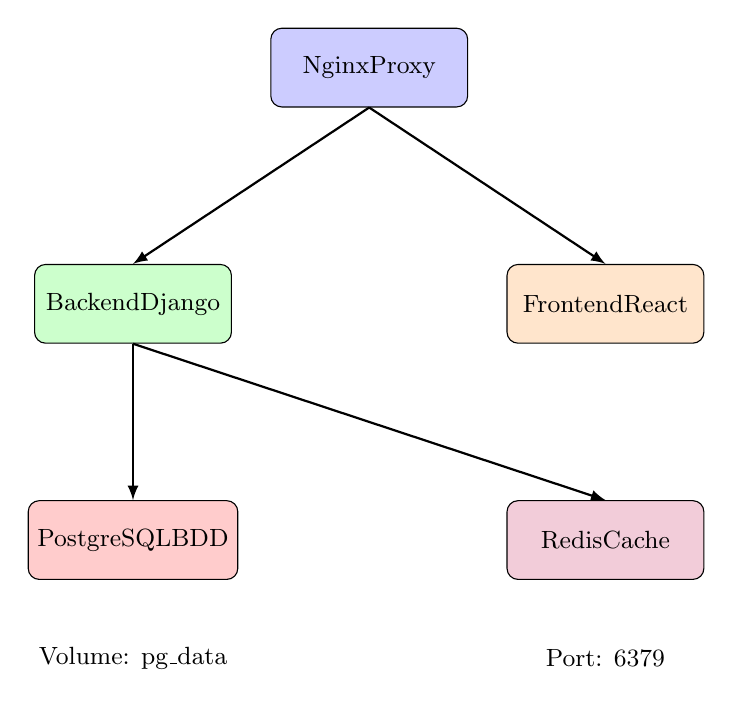
\begin{tikzpicture}[
    svc/.style={rectangle, draw, rounded corners, minimum width=2.5cm, minimum height=1cm, font=\small, text centered},
    link/.style={-latex, thick}
]

% Services
\node[svc, fill=blue!20] (nginx) at (0,3) {Nginx \\ Proxy};
\node[svc, fill=green!20] (backend) at (-3,0) {Backend \\ Django};
\node[svc, fill=orange!20] (frontend) at (3,0) {Frontend \\ React};
\node[svc, fill=red!20] (db) at (-3,-3) {PostgreSQL \\ BDD};
\node[svc, fill=purple!20] (redis) at (3,-3) {Redis \\ Cache};

% Connexions
\draw[link] (nginx.south) -- (backend.north);
\draw[link] (nginx.south) -- (frontend.north);
\draw[link] (backend.south) -- (db.north);
\draw[link] (backend.south) -- (redis.north);

% Légende
\node at (-3,-4.5) {\small Volume: pg\_data};
\node at (3,-4.5) {\small Port: 6379};

\end{tikzpicture}
\caption{Architecture des services Docker de SmartClub Analytics}
\label{fig:docker-arch}
\end{figure}

\section{Conception de la Base de Données}

\subsection{Schéma Relationnel}

La base de données PostgreSQL est organisée selon le schéma relationnel suivant :

\begin{itemize}
    \item \textbf{Table \texttt{players}} : Informations démographiques et statut des joueurs (31 joueurs dans la configuration initiale).
    \item \textbf{Table \texttt{injuries}} : Historique des blessures avec type, sévérité, et dates.
    \item \textbf{Table \texttt{contracts}} : Données contractuelles avec période de validité et salaire.
    \item \textbf{Table \texttt{training\_loads}} : Enregistrements quotidiens de charge d'entraînement.
    \item \textbf{Table \texttt{wellness}} : Scores quotidiens de bien-être (fatigue, sommeil, courbatures).
    \item \textbf{Table \texttt{nutrition\_plans}} : Plans nutritionnels par joueur et par date.
    \item \textbf{Table \texttt{foods}} : Base de données alimentaires importée de FoodData Central USDA.
    \item \textbf{Table \texttt{chat\_sessions}} : Sessions de conversation avec l'assistant IA.
    \item \textbf{Table \texttt{chat\_messages}} : Messages individuels avec historique des appels d'outils.
\end{itemize}

\subsection{Indexation et Performance}

\begin{itemize}
    \item Index composites sur \texttt{(player\_id, date)} pour les requêtes temporelles fréquentes.
    \item Index GIN sur les champs JSON pour les métadonnées flexibles.
    \item Partitionnement mensuel pour les tables de séries temporelles (\texttt{training\_loads}, \texttt{wellness}).
\end{itemize}

\section{Conception des APIs REST}

\subsection{Endpoints Principaux}

\begin{table}[H]
\centering
\begin{tabular}{|c|c|c|l|}
\hline
\textbf{Méthode} & \textbf{Endpoint} & \textbf{Module} & \textbf{Description} \\
\hline
POST & \texttt{/api/token/} & Auth & Obtenir un token JWT \\
POST & \texttt{/api/token/refresh/} & Auth & Rafraîchir le token JWT \\
GET & \texttt{/api/v2/physio/squad/daily-risk} & Physio & Risques quotidiens de l'effectif \\
GET & \texttt{/api/v2/physio/players/profiles} & Physio & Profils physiologiques des joueurs \\
GET & \texttt{/api/v2/physio/timeseries/\{id\}/} & Physio & Série temporelle ACWR d'un joueur \\
POST & \texttt{/api/chat-llm/stream/} & Chat IA & Requête à l'assistant IA (SSE) \\
GET & \texttt{/api/scout/players/} & Scouting & Liste des joueurs avec filtres \\
GET & \texttt{/api/nutrition/foods/} & Nutrition & Recherche dans la base alimentaire \\
POST & \texttt{/api/nutrition/generate-plan/} & Nutrition & Générer un plan nutritionnel \\
\hline
\end{tabular}
\caption{Endpoints REST principaux de SmartClub Analytics}
\label{tab:endpoints}
\end{table}

\subsection{Sérialiseurs Django REST}

Chaque module expose des sérialiseurs pour valider et transformer les données :

\begin{itemize}
    \item \textbf{PlayerSerializer} : Inclut les champs de base, l'âge calculé, et les métriques de risque agrégées.
    \item \textbf{InjuryRiskSerializer} : Combine les données de charge d'entraînement et de bien-être pour calculer un score de risque.
    \item \textbf{ChatMessageSerializer} : Gère le format des messages avec historique des appels d'outils et contexte utilisateur.
    \item \textbf{FoodSerializer} : S'interface avec la base FoodData Central pour la recherche et le calcul nutritionnel.
\end{itemize}

\section{Conception du Module d'Intelligence Artificielle}

\subsection{Agent Conversationnel (Chat LLM)}

L'agent conversationnel est le composant le plus sophistiqué du système. Son architecture repose sur :

\begin{itemize}
    \item \textbf{Orchestrateur d'outils} : Un agent qui reçoit la requête utilisateur, interroge le LLM, exécute les outils demandés, et synthétise la réponse.
    \item \textbf{Tool Registry} : Un catalogue d'outils accessibles au LLM avec leur schéma JSON (paramètres, types, descriptions).
    \item \textbf{Gestion de session} : Conservation de l'historique des conversations avec élagage automatique pour respecter les limites de tokens.
    \item \textbf{Support multilingue} : Prompts système adaptés à chaque langue (français, anglais, arabe, dialecte tunisien).
\end{itemize}

\subsection{Modèles de Prédiction (Machine Learning)}

\begin{itemize}
    \item \textbf{Modèle de prédiction d'absence} : Utilise des caractéristiques de charge d'entraînement et de bien-être sur une fenêtre glissante de 28 jours pour prédire les absences à 7 jours.
    \item \textbf{Modèle de risque de blessure} : Combine ACWR, fatigue, qualité du sommeil, et historique des blessures dans un ensemble Random Forest.
    \item \textbf{Métrique ACWR} : Calculée comme le ratio entre la charge aiguë (moyenne mobile sur 7 jours) et la charge chronique (moyenne mobile sur 28 jours).
\end{itemize}

\section{Architecture de Sécurité}

\subsection{Authentification et Autorisation}

\begin{itemize}
    \item \textbf{JWT (JSON Web Token)} : Authentification sans état avec tokens d'accès (24h) et de rafraîchissement (7 jours).
    \item \textbf{RBAC (Role-Based Access Control)} : Quatre rôles distincts avec des permissions granulaires :
    \begin{itemize}
        \item \textbf{Admin} : Accès complet à toutes les fonctionnalités et à la gestion des utilisateurs.
        \item \textbf{Coach/Entraîneur} : Accès aux données de performance, scouting, et assistant IA.
        \item \textbf{Physio} : Accès aux données physiologiques, risque de blessure, et nutrition.
        \item \textbf{Manager} : Accès aux données contractuelles et aux rapports de scouting.
    \end{itemize}
    \item \textbf{Protection CSRF} : Tokens CSRF pour toutes les requêtes mutatives (POST, PUT, DELETE).
    \item \textbf{Sécurisation des endpoints API} : Validation des permissions via des décorateurs Django REST personnalisés.
\end{itemize}

\section{Diagramme de Déploiement}

\subsection{Infrastructure Cible}

\begin{figure}[H]
\centering
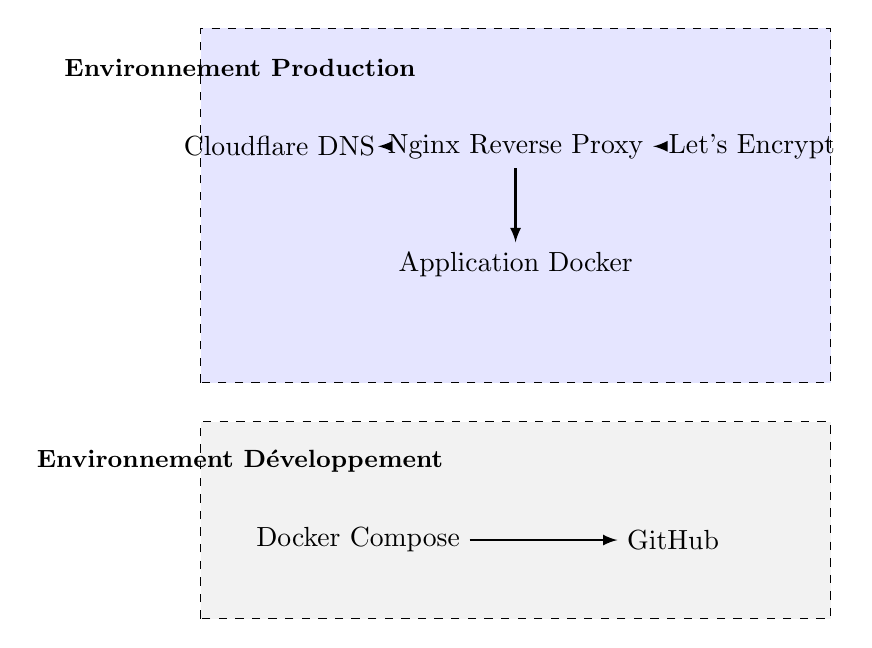
\begin{tikzpicture}[
    node/.style={rectangle, draw, rounded corners, minimum width=2.5cm, minimum height=0.8cm, font=\small, text centered},
    link/.style={-latex, thick}
]

% Environnements
\draw[fill=blue!10, dashed] (-4, 1.5) rectangle (4, 6);
\node at (-3.5, 5.5) {\small \textbf{Environnement Production}};

\draw[fill=gray!10, dashed] (-4, -1.5) rectangle (4, 1);
\node at (-3.5, 0.5) {\small \textbf{Environnement Développement}};

% Nœuds Production
\node (nginx) at (0, 4.5) {Nginx Reverse Proxy};
\node (app) at (0, 3) {Application Docker};
\node (cert) at (3, 4.5) {Let's Encrypt};
\node (dns) at (-3, 4.5) {Cloudflare DNS};

% Nœuds Développement
\node (local) at (-2, -0.5) {Docker Compose};
\node (git) at (2, -0.5) {GitHub};

% Connexions
\draw[link] (nginx) -- (app);
\draw[link] (cert) -- (nginx);
\draw[link] (dns) -- (nginx);
\draw[link] (local) -- (git);

\end{tikzpicture}
\caption{Diagramme de déploiement de SmartClub Analytics}
\label{fig:deployment}
\end{figure}

\section{Conclusion}

Ce chapitre a présenté la conception détaillée de SmartClub Analytics à travers des diagrammes UML, des modèles de données, et des architectures de composants. La conception en couches (présentation, API, métier, données) assure une séparation claire des responsabilités et facilite la maintenance et l'évolution du système. Le chapitre suivant détaillera l'implémentation concrète de ces composants.
